In this section we present our data on the expected number of ballots drawn as the number of rounds increases, and on the fraction of audits that stop (an estimate of cumulative stopping probability, $C_j$) for the states of Texas, Missouri and Massachusetts, with margins of $0.057$, $0.157$ and $0.342$ respectively. Interestingly, we observe that $\Minerva$ has an advantage for a first round size with stopping probability $S_1=0.25$, but it is not as large as that for $S_1=0.9$. On all our plots we mark ASN, the Average Sample Number for B2 \BRAVO for context. Notice that, in all the plots, both instances of \Minerva show a higher probability of completion than does either \BRAVO audit when the average number of ballots drawn is ASN. 

\begin{figure}
\begin{centering}
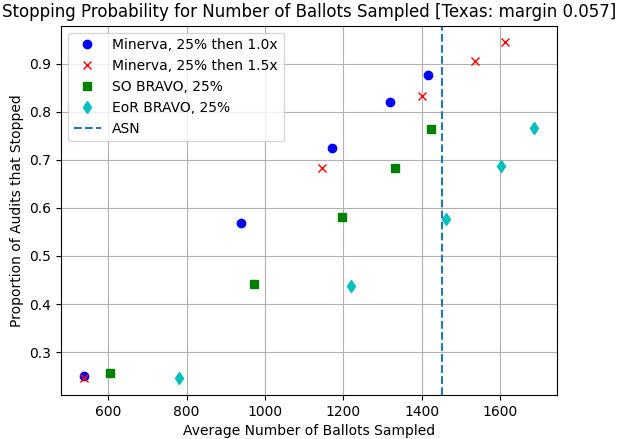
\includegraphics[width=0.6\textwidth]{texas25.png}
\caption{This plot shows the cumulative fraction of audits that stopped as a function of average number of sampled ballots for all four audits we studied, for the state of Texas, margin $0.057$, and first round stopping probability $S_1=0.25$.}
\label{fig:texas_25}
\end{centering}
\end{figure}

We observe that the behavior of both \Minerva audits is similar, and that the plot for SO \BRAVO is to the right of (more ballots) and below (lower probability of stopping) those for \Minerva, even for a stopping probability as low as $0.25$. We observe that the plot for EoR \BRAVO shows the worst performance, which is not surprising. We observe similar behavior across margins (see Figures \ref{fig:missouri_25} and \ref{fig:mass_25}), though the improvement due to \Minerva reduces as margins get larger. We see also that the improvement due to using \Minerva is not as large as that seen for $S_1=0.9$ (see Figure \ref{fig:texas_90}). 

For $S_1=0.25$, the ratio of first round size of EoR \BRAVO to \Minerva is $1.45$, $1.37$, $1.23$ for states Texas, Missouri and Massachusetts, and margins $0.057$, $0.157$ and $0.342$ respectively. This may be compared to $2.03$, $1.99$ and $1.8$ respectively for $S_1=0.9$. Similarly, for $S_1=0.25$, the ratio of first round size of SO \BRAVO to \Minerva is $1.13$, $1.08$, $1.12$ for states Texas, Missouri and Massachusetts, and margins $0.057$, $0.157$ and $0.342$ respectively. This may be compared to $1.38$, $1.38$ and $1.30$ respectively for $S_1=0.9$. Note that the effect of such improvements on workload depends greatly on the number of ballots being sampled. For example, a $20\%$ reduction in sample size in Massachusetts might save election officials $10$ ballots, whereas the same reduction in Texas could save thousands.

\begin{figure}
\begin{centering}
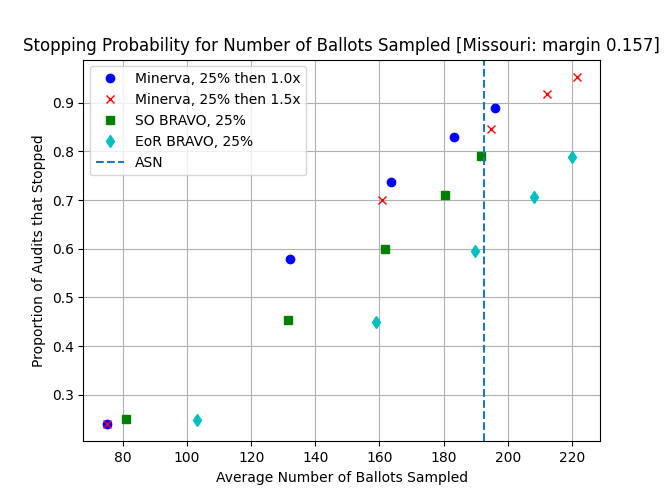
\includegraphics[width=0.65\textwidth]{missouri25.png}
\caption{This plot shows the cumulative fraction of audits that stopped as a function of average number of sampled ballots for all four audits we studied, for the state of Missouri, margin $0.157$, and first round stopping probability $S_1=0.25$.}
\label{fig:missouri_25}
\end{centering}
\end{figure}

\begin{figure}
\begin{centering}
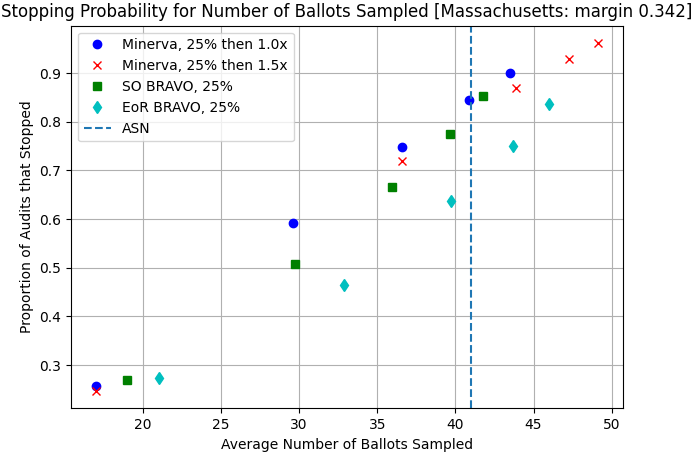
\includegraphics[width=0.65\textwidth]{massachusetts25.png}
\caption{This plot shows the cumulative fraction of audits that stopped as a function of average number of sampled ballots for all four audits we studied, for the state of Massachusetts, margin $0.342$, and first round stopping probability $S_1=0.25$.}
\label{fig:mass_25}
\end{centering}
\end{figure}

\begin{figure}
\begin{centering}
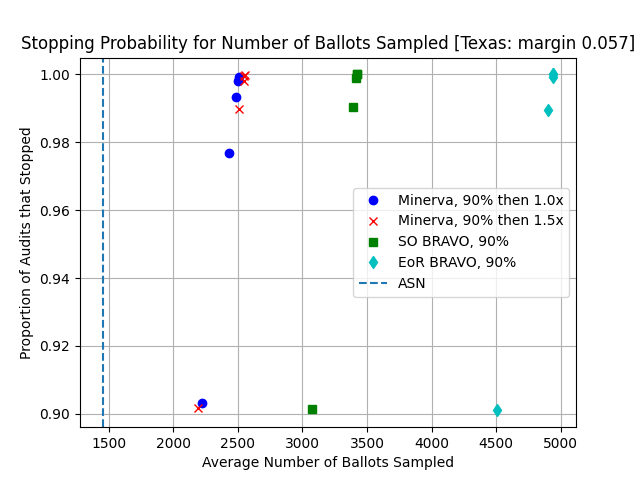
\includegraphics[width=0.605\textwidth]{texas90.png}
\caption{This plot shows the cumulative fraction of audits that stopped as a function of average number of sampled ballots for all four audits we studied, for the state of Texas, margin $0.057$, and first round stopping probability $S_1=0.9$.}
\label{fig:texas_90}
\end{centering}
\end{figure}

